\chapter{技术路线}

\section{相关工作}
\subsection{HOF特征和CSS特征+HIKSVM分类器\cite{walk2010new}}{
该研究以多种方式推动了行人检测的最新技术:该研究已经为行人检测引入了强大的自相似特征,当应用于色彩通道时,在单帧设置和附加运动信息方面提供了显着的改进。精心实现的HOG特征,HOF特征图像运动的变体和新的CSS特征以及HIKSVM作为分类器的组合,超过了之前技术5%-20%的的精度。
}

\subsection{积分通道特征\cite{integral}}{
积分通道特征的大概思路是:通过对输入图像做各种线性和非线性的变换,诸如局部求和、直方图、haar-like及它们的变种之类的特征便可以通过积分图来快速计算出来。给定一个输入图像I,其所对应的通道是原始输入图像的某种输出响应。对于灰度图而言,其对应的通道C=I。而对于彩图而言,其每个颜色通道则对应一个通道。其他类似的通道可以通过各种线性和非线性的方法计算而来。令$\Omega$代表图像的某种通道计算函数,则,$C=\Omega(I)$。为了能利用滑动窗口快速计算,通道应该具有变换不变性,即,对于原图I及其对应的某种变换$I'$而言,$C=\Omega(I)$和$C'=\Omega(I')$应该成立,如此一来,便允许$\Omega$在整个图像上计算一次,从而避免了变换之后的重复计算。
\begin{figure}[htbp]
\centering
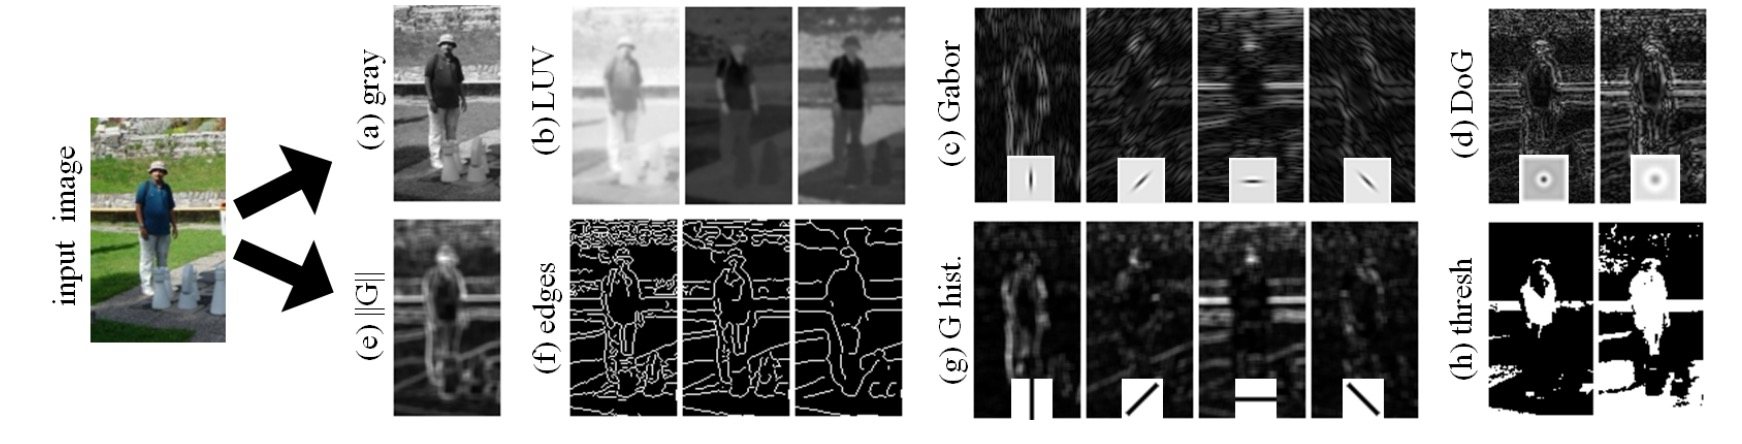
\includegraphics[width=5in]{images/JFTD.png}
\caption{积分通道特征}
\label{JFTD}
\end{figure}
}

\subsection{Faster R-CNN\cite{faster}}{
Faster R-CNN(其中R对应于“Region(区域)” )是基于深度学习R-CNN系列目标检测最好的方法。使用VOC2007+2012训练集训练,VOC2007测试集测试mAP达到73.2\%,目标检测的速度可以达到每秒5帧。
技术上将RPN网络和Fast R-CNN网络结合到了一起,将RPN获取到的proposal直接连到ROI pooling层,是一个CNN网络实现端到端目标检测的框架。
\begin{figure}[htbp]
\centering
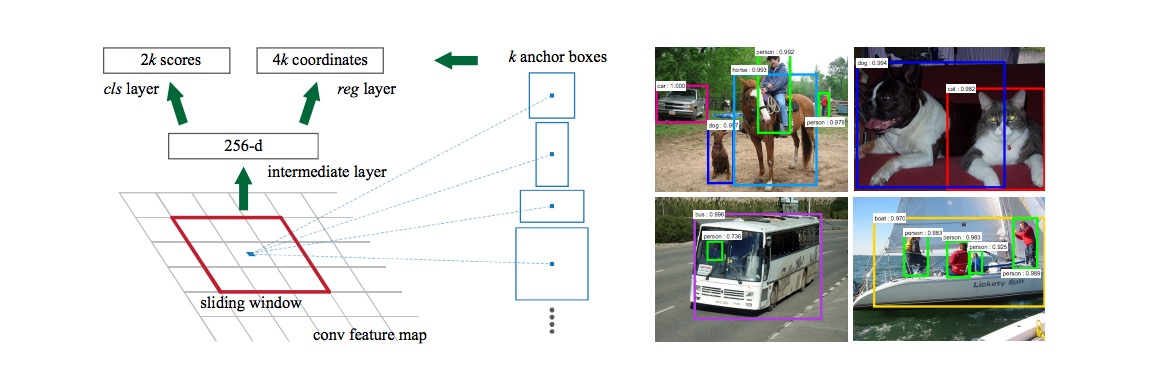
\includegraphics[width=5in]{images/Faster.png}
\caption{Faster R-CNN}
\label{Faster}
\end{figure}
}

\subsection{SSD\cite{ssd}}{
SSD也是一种深度学习的神经网络方法。它将原网络后再加入几层特征卷积层,原全联接层提取的特征进入特征提取层,能提取原图各个尺度的特征,通过这些特征计算出检测的物体。
\begin{figure}[htbp]
\centering
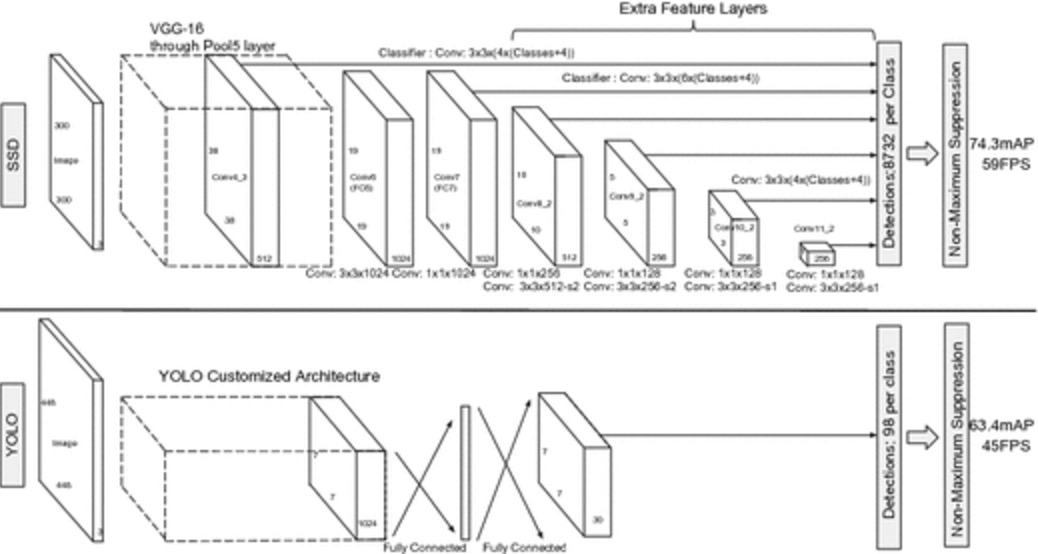
\includegraphics[width=5in]{images/SSD.png}
\caption{SSD网络模型}
\label{SSD}
\end{figure}
}

\subsection{YOLO\cite{yolo}}{
YOLO将对象检测重新映射为单个回归问题,直接从图像像素到边界框坐标和类概率。YOLO将预测该物体是什么对象以及它在什么位置。

YOLO非常简单:单个卷积神经网络同时预测了这些框的各个边界框和类概率。YOLO通过完整的图片训练,直接优化检测性能。 这种统一的模型比传统的对象检测方法有好几个好处。

首先,YOLO非常快。 由于YOLO将框检测作为回归问题,YOLO不需要复杂的流水线。

第二,YOLO在做出预测时,会全局地推理图片信息。 与滑动窗口和基于区域提案的技术不同,YOLO在训练和测试时间期间处理整个图像,因此它可以编码关于类及其外观的语义信息。

第三,YOLO的泛华性更强。
\begin{figure}[htbp]
\centering
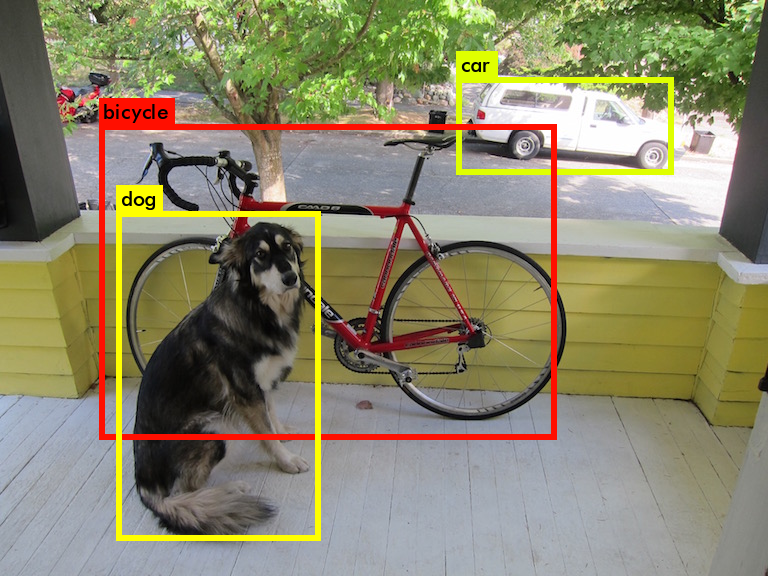
\includegraphics[width=5in]{images/YOLO.png}
\caption{YOLO检测}
\label{YOLO}
\end{figure}
}

\section{关键技术}{
	\begin{figure}[htbp]
	\centering
	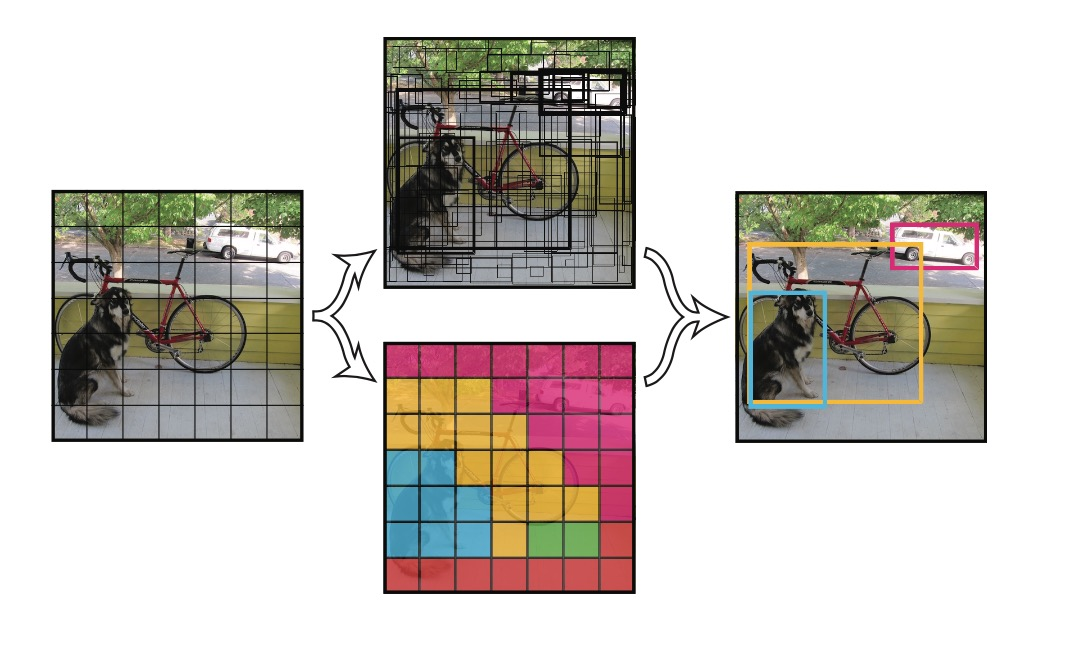
\includegraphics[width=5in]{images/YOLOMX.png}
	\caption{YOLO模型}
	\label{YOLOMX}
	\end{figure}
	YOLO将对象检测的单独组件统一为单个神经网络。YOLO网络使用整个图像的特征来预测每个边界框。它还同时预测图像的所有边界框。这意味着YOLO的网络全局地推断整张图像和所有对象。

	如图\ref{YOLOMX},YOLO将整个输入图像分为S×S格。如果物体的中心落入网络单元格中,则该网络单元负责检测该对象。

	每个网格单元预测B边界框和置信度分数。这些置信度分数反映了模型对于框包含对象的概率,以及它认为边界框预测的准确程度。我们将置信度定义为$Pr(Obeject)*IOU_{pred}^{truth}$。如果该单元格中没有对象,则置信度分数应为零。 否则,我们希望置信度分数等于预测框和真值之间的交集(IOU)。

	每个边界框包括5个预测:x,y,w,h和置信度。(x,y)坐标表示相对于网格单元边界的框的中心。从整个图像预测宽度和高度。 最后置信度预测表示预测框和任何真值框之间的IOU。

	每个网格单元还预测了C类的条件概率,$Pr(Class_i|Object)$。 这些概率在包含物体的网格单元格上被约束。 我们只预测每个网格单元的一组类概率,而不考虑框的数量B。

	在测试的时候,我们乘以类的条件概率和单独的框置信度,$Pr(Class_i|Object)*Pr(Object)*IOU_{pred}^{truth}=Pr(Class_i)*IOU_{pred}^{truth} (1)$这给了我们每个边界框的特定类的置信分数。 这些分数对该类出现在框中的概率进行了编码,并且预测框有多符合该物体。
}

\section{项目框架}{
	Darknet\cite{darknet}是一个基于C语言和CUDA的开源神经网络框架。它支持CNN、RNN、YOLO等各种神经网络。YOLO作者使用的框架,同时也是YOLO效果最好的框架。Darknet支持GPU加速,支持OpenCV,同时由于它是个轻量级的框架配置较为方便,各个操作系统也都能配置,可移植性强。同时本项目是基于YOLO的网络结构的实验,所以选择了Darknet作为本项目的实验框架。
}

\section{KITTI数据集}{
	KITTI\cite{KITTI}利用自主驾驶平台Annieway来开发新的具有挑战性的现实世界的计算机视觉基准。KITTI感兴趣的任务是:立体声,光流,视觉测距,3D物体检测和3D跟踪。为此,KITTI配备了两台高分辨率彩色和灰度摄像机的标准车厢。 Velodyne激光扫描仪和GPS定位系统提供了准确的地面实况。卡尔斯鲁厄市中心的农村地区和高速公路上都是通过驾驶卡车来捕捉的。每张图片最多可显示15辆汽车和30名行人。除了以原始格式提供所有数据,KITTI提取每个任务的基准。对于我们的每个基准,KITTI还提供评估指标和评估网站。初步实验表明,在实验室迁移到现实世界之前,诸如米德尔伯里等已建立基准的方法排名高于平均水平。我们的目标是通过向社会提供新的困难的现实基准,来减少这种偏差并补充现有的基准。

	KITTI包含市区、乡村和高速公路等场景采集的真实图像数据,每张图像中最多达15辆车和30个行人,还有各种程度的遮挡与截断。整个数据集由389对立体图像和光流图,39.2 km视觉测距序列以及超过200k 3D标注物体的图像组成 ,以10Hz的频率采样及同步。总体上看,原始数据集被分类为’Road’, ’City’, ’Residential’, ’Campus’ 和 ’Person’。对于3D物体检测,label细分为car, van, truck, pedestrian, pedestrian(sitting), cyclist, tram以及misc组成。
}

\section{本章小结}{
	本章主要介绍了之前的一些研究工作。接着描述了本项目的关键技术,然后介绍了本项目的框架Darknet,最后简单介绍了本项目的数据集KITTI。

	基于本项目的需求:性能、速度。本项目将参考YOLO的网络结构,在Darknet上进行网络的训练和测试,使用KITTI数据集作为我们训练和测试的数据集。
}
